%&program=xetex
%&encoding=UTF-8 Unicode

% thesis.tex

\documentclass[12pt]{report}
\usepackage{pdfpages}
\usepackage{tikz}
\usepackage{pgfplots}
\usepackage{utepcsthesis}
\usepackage{graphics}
\usepackage{amsmath}
\usepackage{amssymb}
\usepackage[top=1.0in,bottom=1.0in,left=1.25in,right=1.25in]{geometry}
\usepackage{longtable}
\usepackage{setspace}
\usepackage{booktabs}
\usepackage{listings}
\usetikzlibrary{shadows,arrows}
%\usepackage[T1]{fontenc}
%     \usepackage{txfonts}
\usepackage{mathptmx}


% \usepackage{marvosym}
% \usepackage{fontspec}   %load fonts
% \usepackage{url,parskip}   %formatting
% \usepackage{xunicode,xltxtra}  %other packages for XeTeX
% \usepackage{titlesec}
\usepackage{amsmath,amsfonts}






% \font\title="Lohit Tamil:script=taml" at 22pt


% \renewcommand{\encodingdefault}{T1}
% \renewcommand{\rmdefault}{tnr}
% \usepackage{mathptmx}
\usepackage{hyperref}
% \usepackage[LY1]{fontenc}
% \usepackage{timesnewx} 
\begin{document}
% \rmfamily{Time}
% 		%%%%%%%%%%%%%%%%%%%%%
% 		% Preliminary Pages %
% 		%%%%%%%%%%%%%%%%%%%%%%%%%%%%%%%%%%%%%%%%%%%%%%%%%%%%%%%%%%%%%%%%%%%%%%%%%%%%%%%%

% 		% Set the table of contents depth (tocdepth) to the least significant section
% 		% type that you want to be included in the table of contents using this key:
% 		%   1 = section
% 		%   2 = subsection
% 		%   3 = subsubsection
% 		%   4 = paragraph
% 		\setcounter{tocdepth}{2}

% 		% The graduate school requires all caps for the title, and if
% 		% the title contains more than one line, the lines should be
% 		% of decreasing length, giving the look of an inverted pyramid.

% 		\title{CS 491\\[0.4in]Optical Character Recognition (OCR) for Tamil Language}
% 		% If the title is more than one line, separate the lines with \\[1pc]
% 		% as shown below:
% 		%\title{THIS IS THE VERY FIRST LINE\\[1pc]
% 		%       THIS IS THE SECOND LINE\\[1pc]
% 		%       THIS IS THE THIRD ONE}

% 		% The author should also be all caps
% 		\author{PRADEEP M,          CB.EN.U4CSE08131}
% 		% Uncomment to put degrees on title page
% 		%\AuthorDegrees{B.S.}
% 		\date{November 2011}
% 		\DeptName{Computer science and Engineering, School of Engineering, Amrita Vishwa Vidyapeetham}

% 		\CommitteeChair{Shanmuga Velayudam, Chair, Ph.D.}
% 		\CommitteeMembers{Hema P Menon, M.Tech.}
% 				 {Praveen Krishnan, M.Tech.}
% 		%Uncomment if you have a fourth member on your committee
% 		%\AdditionalMember{Additional Member's name}

% 		\GradSchoolDean{P N Kumar, MBA.}

% 		%Produce the signature page
% 		\makesigpage

% 		%Uncomment if you want a copyright page
% 		\begin{CenteredPage}
% 		\copyright Copyleft\\[0.2in]
% 		by\\[0.2in]
% 		Pradeep M\\[0.2in]
% 		2011
% 		\end{CenteredPage}

% 		%Delete if you don't want a dedication
% 		\begin{CenteredPage}
% 		{\it to the\\[0.2in]
% 		world\\[0.2in]
% 		}
% 		\end{CenteredPage}

%\maketitlepage
% % \addcontentsline{toc}{chapter}{}

% \chapter*{}
OCR FOR TAMIL
LANGUAGE



PROJECT REPORT SUBMITTED BY,

PRADEEP.M 
pradeepmadesh@gmail.com




   


% \usepackage{pdfpages}
% \begin{document}
% \includepdf[pages=-]{1.pdf}
% \includepdf[pages=-]{2.pdf}
% \includepdf[pages=-]{3.pdf}
% \end{document}
% \includepdf[pages={1}]{myfile.pdf}
%     \documentclass{article}
%     \usepackage{pdfpages}
%     \begin{document}
%     \includepdfmerge{file1.pdf,-}
%     \includepdfmerge{file2.pdf,1-3}
%     \end{document}
% \addcontentsline{toc}{chapter}{}

% \chapter*{}
\begin{center}
 %\onehalfspacing
%  \doublespacing

% \documentclass[a4paper,10pt]{article}
% \usepackage{fix-cm}
% \begin{document}
% \fontsize{60}{70}\selectfont Huge text
% \end{document}
%  \def\Large{ \font\Tinyfont = cmr10 at 16pt \relax  \Tinyfont}
\Large{
\textbf{ 
OCR FOR TAMIL LANGUAGE  
}
}
\begin{spacing}{2.0}
\end{spacing}
\onehalfspacing

\large{A PROJECT REPORT \\
\textbf{ \emph{submitted by}} \\
}
\Large{
PRADEEP M  \\
(CB.EN.U4CSE08131) \\
\textbf{
\emph{in partial fulfillment for the award of the degree\\ of\\}
}
}
\large{
BACHELOR OF TECHNOLOGY \\
IN \\
COMPUTER SCIENCE AND ENGINEERING \\ 
% \begin{picture}(12,12)(0,0)
% \put(1.5,1.5){a}
% \put(4,4){\circle{8}}
% \end{picture}

 \begin{spacing}{2.0}
\end{spacing}
\includegraphics[scale=0.5]{./img/am_logo}
\begin{spacing}{2.0}
\end{spacing}

AMRITA SCHOOL OF ENGINEERING, COIMBATORE\\
}
\Large{AMRITA VISHWA VIDYAPEETHAM} 
\\
COIMBATORE – 641 112	  \\
%\onehalfspacing
\begin{spacing}{2.0}
\end{spacing}
\large{
APRIL 2012
}
\end{center}   
 % \addcontentsline{toc}{chapter}{}

% \chapter*{}
%\renewcommand{\rmdefault}{Calibri}
% \setstretch{1.8}
%\onehalfspacing 
%Signature\hspace{0.5cm} \makebox[1.5in]{\hrulefill}
\begin{center}
\large{\textbf{ AMRITA VISHWA VIDYAPEETHAM \\ AMRITA SCHOOL OF ENGINEERING, COIMBATORE \\ 
\begin{spacing}{2.0}
\end{spacing}
\includegraphics[scale=0.5]{./img/am_logo} 
\begin{spacing}{2.0}
\end{spacing}
BONAFIDE CERTIFICATE 
}}
\end{center}
\paragraph{}
%  \doublespacing 
\begin{spacing}{2.0}
This is to certify that the project report entitled\textbf{ "OCR FOR TAMIL LANGUAGE"}, submitted by  \textbf{"PRADEEP M","RegNo.CB.EN.U4CSE08131"} in partial fulfillment of the requirements for the award of the degree of Bachelor of Technology in  \textbf{"COMPUTER SCIENCE AND ENGINEERING"} is a bonafide record of the work carried out under my guidance and supervision at Amrita School of Engineering, Coimbatore.
\end{spacing}
% \singlespacing




\begin{spacing}{2.0}
\end{spacing}
\hfill \\
% SIGNATURE \hfill SIGNATURE \\
Mrs. HEMA P MENON,  \hfill	                                    Dr. K P SOMAN, \\
Project Advisor,         \hfill                                             External Advisor,\\
Assistant Professor, CSE					   \hfill   Professor, CEN 
\begin{spacing}{2.0}
\end{spacing}
\hfill \\
Chairperson, CSE \\
Prof. P N KUMAR \\
% \raggedright{}
% \doublespacing


\begin{center}
% Submitted for the university examination held on ...............
This project report was evaluated by us on ..............................
\end{center}
% \parbox{15cm}{signature one\\signature two}
% \textbf{ 
% \begin{flushleft}
% INTERNAL EXAMINER 
% \begin{flushright}
% EXTERNAL EXAMINER 
% \end{flushright}
% \end{flushleft}	    		                            
% }
\begin{spacing}{2.0}
\end{spacing}
 INTERNAL EXAMINER \hfill EXTERNAL EXAMINER    
%  % \addcontentsline{toc}{chapter}{}

% \chapter*{}

AMRITA VISHWA VIDYAPEETHAM

AMRITA SCHOOL OF ENGINEERING,
COIMBATORE

COMPUTER SCIENCE AND ENGINEERING      


DECLARATION

I, PRADEEP.M (RegNo.CB.EN.U4CSE08131) hereby declare that this project report, entitled "OCR FOR TAMIL LANGUAGE", is a record of the original work done by me under the guidance of Mrs. HEMA P MENON,Assistant Professor, CSE,  Dr. K P SOMAN, Professor, CEN, and Dr. M SABARIMALAI MANIKANDAN, Assistant Professor, CEN, Amrita School of Engineering, Coimbatore and that this work has not formed the basis for the award of any degree / diploma / associate ship / fellowship or a similar award, to any candidate in any University, to the best of my knowledge.



Place:
Date:                                                                                                                  PRADEEP.M


COUNTERSIGNED


Dr P N KUMAR
Head of the Department
Computer Science and Engineering   
% acknowl.tex {Acknowledgements}

\addcontentsline{toc}{chapter}{Acknowledgements}

\chapter*{Acknowledgements}
% \paragraph{}
% First of all, I am grateful to the entire academic community and many others for nurturing me over the
% course of four years.
% \paragraph{}

\paragraph{}
I would like to thank my project advisors namely, Mrs. Hema P Menon and 
Dr. K P Soman for their advice and patience.
\paragraph{}
I also extend my gratitude to Professor. P N Kumar, Chairperson, CSE. 
I would like to thank our project co-ordinators namely Mr. M Senthtil Kumar, Mr. A K Sumesh and 
Mr. R Gowtham.
\paragraph{}
I also want to thank my collaborator Mr. Praveen Krishnan for providing help and sharing his experience on working in Tamil OCR. I also owe my thanks to parents and friends. In addition, I would like to thank Dr. Sabarimalai Manikandan for giving me an opportunity to work in Tamil OCR.
\paragraph{}
Finally I want to thank the Almighty.       % Acknowledgements, optional
%\include{preface}       % Preface, optional
\addcontentsline{toc}{chapter}{Abstract}

\chapter*{Abstract}

%\{Optical Character Recognition (OCR)}


% \begin{abstract}
%\begin{center}
%Optical Character Recognition (OCR) for Tamil language\\[0.2in]
%\end{center}
% OCR is robust for many European languages but it is not the case for Indic languages. 
% So the main goal of our work is to increase the robustness especially for Tamil language. 
% We could use the existing OCR like Tesseract or Ocropus but we found that it is not suitable
% for Tamil language. Moreover, the algorithms used in these OCR systems are not start-of-the-art 
% so we want to apply the latest algorithms and find out how good is the result. 
% We are dissecting the entire OCR system right from preprocessing to postprocessing.
% Our objective is to use this OCR system to create parallel corpus for Machine Translation 
% and possibly creating electronic encyclopedia from existing old documents. 
% \end{abstract}
\begin{spacing}{1.5}
Optical Character Recognition (OCR) system is robust for Latin languages but it is not so for Indic languages. It is partly because of the number of character classes and close similarity of characters.

In this work, we are presenting a comparative study of recognition based on supervised and 
unsupervised learning. The former is based on SVM based training and classification (SVMTC) and the
later is based on Random Projection Technique (RPT). The challenging part of this project 
is feature  extraction. We have extracted features based on active contour model, 
character geometry, moment invariants, random projection and Gabor filter. It is a combination of 
statistical and visual features. Overall, RPT gives better results than
SVMTC. The result based on RPT is found out to be 58 \%.
\end{spacing}

      % Abstract, optional, but strongly recommended

\tableofcontents        % Generate Table of Contents

% If you a list of tables, uncomment the next line.
% It is required if the document contains three or more tables
\listoffigures
\listoftables
 \addcontentsline{toc}{chapter}{List of Abbreviations}

\chapter*{List of Abbreviations}
% \begin{center}
\begin{spacing}{1.5}
ACM - Active Contour Model \\
OCR - Optical Character Recognition \\
PCA - Principal Component Analysis \\
QP - Quadratic Programming \\
RPT - Random Projection Technique \\
SDT - Shape Derivative Tool \\
SVMTC - SVM based training and classification \\
WWW - World Wide Web \\

\end{spacing}
% \end{center}
 
% If you use a list of figures, uncomment the next line
% It is required if the document contains three or more figures



% Here would go optional list of illustrations, maps, slides

%%%%%%%%
% Body %
%%%%%%%%%%%%%%%%%%%%%%%%%%%%%%%%%%%%%%%%%%%%%%%%%%%%%%%%%%%%%%%%%%%%%%%%%%%%%%%%

%Start arabic numbering, bottom of first page and top right of subsequent pages
\StartBody
\begin{spacing}{1.5}
\chapter{Introduction}

\section{Optical character recognition system}
OCR system is a software which recognizes text in a document image. It does document 
image analysis in order to recognize a piece of text. Some of the applications of OCR system is
discussed in the last chapter. It involves the area of image processing and pattern recognition.
It also proves to be a great aid to the machine translation system by
capturing the raw corpus from multilingual books\cite{praveen}. It can also extract text from
videos by doing document image analysis on the relevant frames in the video.

\section{Challenges}
The main challenge lies in tackling touching characters and 
recognizing characters which are almost similar. 
\section{Tamil Character Set}
Tamil is a Dravidian language spoken in Tamil Nadu, India, North eastern Sri Lanka, Singapore and  Malaysia. The language has 31 basic alphabets (12 vowels, 18 consonants and a special consonant) and the written script is comprises of 247 characters. However for character recognition there are only 155 classes which can be refered in \ref{CSET} including grantha characters. But this number excludes Tamil numerals which are uncommon.


\section{Previous work}
Previously Dr V. Krishnamoorthy, proposed a OCR system for Tamil language. 
The author claims 99\% accuracy on printed text\cite{krish}. Later, Anbumani Subramanian and Bhadri Kubendran et.al proposed a system\cite{anbu}. Again, it also claims better result. Both of the system doesn't perform page layout analysis and the system is no longer maintained. These systems uses moment based feature extraction technique. 
\paragraph{}
In 2005, \cite{seetha} proposed a system which did 
a comparative analysis of ANN and SVM for learning and classification. The SVM based classifier claims an accuracy of 66\% for single font. They used the following 
visual features which is based on character glyph.
\begin{itemize}
\item Height of the character
\item  Width
of the character
\item Numbers of horizontal lines
\item Numbers of vertical lines
\item Numbers of circles
\item Numbers of horizontally oriented arcs
\item Numbers of vertically oriented arcs
\item Centroid of
the image
\item Position of the various features
\item Pixels in the various regions
\end{itemize}


In 2008,\cite{jaga1} proposed a OCR system which augments the power of ANN, SVM and HMM by fusing all of these together. 
In 2009, \cite{jaga2} did a comparative study of same recognition method. This system again uses character glyph based features. However, the author discussed recognition results only for selected number of character classes and the accuracy varies between 88\% to 99\%.
         % Introductory Chapter
\chapter{System Architecture}
\section{Chapter Organisation}
Preprocessing is discussed in the next chapter. Feature extraction, classification and recognition are discussed in the successive chapters. Finally we discuss the results and tools used along with our implementation of recognition engine based on supervised and unsupervised learning.
\section{Architecture}
System architecture shows the steps involved in the analysis of document image.
The architecture of OCR system comprises of six stages and is shown in \ref{OCRA}.

\tikzstyle{materia}=[draw, fill=blue!20, text width=6.0em, text centered,
  minimum height=1.5em,drop shadow]
\tikzstyle{practica} = [materia, text width=18em, minimum width=10em,
  minimum height=3em, rounded corners, drop shadow]

\tikzstyle{materiai}=[draw, fill=green!20, text width=6.0em, text centered,
  minimum height=1.5em,drop shadow]
\tikzstyle{practicai} = [materiai, text width=18em, minimum width=10em,
  minimum height=3em, rounded corners, drop shadow]

\tikzstyle{line} = [draw, thick, color=black!50, -latex']
\newcommand{\practica}[2]{node (p#1) [practica]
  {Step #1\\{\large\textit{#2}}}}

\newcommand{\practicai}[2]{node (p#1) [practicai]
  {Step #1\\{\large\textit{#2}}}}

  \begin{figure}\centering
\begin{tikzpicture}[scale=0.7,transform shape]
 
  % Draw diagram elements
  \path \practica {1}{Page layout analysis};
  \path (p1.south)+(0.0,-2) \practica{2}{Noise removal and binarization};
  \path (p1.south)+(0.0,-4) \practica{3}{Skew correction};
  \path (p1.south)+(0.0,-6) \practica{4}{Segmentation};
  \path (p1.south)+(0.0,-8) \practicai{5}{Classification};
  \path (p1.south)+(0.0,-10) \practicai{6}{Recognition};
  \path (p1.south)+(0.0,-12) \practica{7}{Format reconstruction};
    \path [line] (p1.south) -- node [above] {} (p2) ;
    \path [line] (p2.south) -- node [above] {} (p3) ;
    \path [line] (p3.south) -- node [above] {} (p4) ;
    \path [line] (p4.south) -- node [above] {} (p5) ;
    \path [line] (p5.south) -- node [above] {} (p6) ;
    \path [line] (p6.south) -- node [above] {} (p7) ;
%   \path (p3.south)+(5.0,-1.0) \practica{4}{Amplificador para HF};
  \end{tikzpicture}
    \caption{Architecture of a typical OCR system}\label{OCRA}
\end{figure}

% \section{Preprocessing}
% Preprocessing is carried out by the tesseract engine. It gives bounding box information. 
% Later, it used blob extraction and preprocessing tool. 

\section{Deliverables}
\subsection{RPT}
\begin{itemize}
\item Ground truth generating tool - train.py 
\item Blob extraction and preprocessing - createb.py
\item Recognition engine - hyperplane2.py - our unsupervised classifier
\item Result analyzer - confuse.sh 
\end{itemize}
\subsection{SVMTC}
\begin{itemize}
\item Feature extractor - roger.m 
\end{itemize}         % Chapter 2
\chapter{Preprocessing}
\begin{figure}\centering
\includegraphics[scale=1]{./img/input}
  \caption{Sample image that is fed to tesseract}\label{INPUT}
\end{figure}
\section{Gray scale conversion}
In grayscale conversion, 24-bit image is converted into 8-bit representation
The input image to be recognised is converted into grayscale using the following formula.
\begin{equation}
I = 0.3R + 0.59G + 0.11B
\end{equation}
where R,G,and B corresponds to red, green and blue intensities respectively.
\begin{figure}\centering
\includegraphics[scale=0.3]{./img/gray}
  \caption{Sample gray scale blob}\label{GRAY}
\end{figure}
\section{Thresholding}
Thresholding refers to the pixel intensity to be used for binarization. For example, if threshold value is 
120, all the pixels having value less than 120 are made zero and the rest as one for binary scale conversion.
\section{Image Binarization}
A binary image is a 2-bit representation of an image. Generally  Otsu's thresholding algorithm 
or sauvola algorithm is used to binarize an image. But it  all depends on the document.
\begin{figure}\centering
\includegraphics[scale=0.3]{./img/bin}
  \caption{Sample binary scale blob}\label{BIN}
\end{figure}
\section{Skew Detection and Correction}
Generally, scanned document has to be skew-corrected because of incorrect orientation of 
document while scanning. There are various algorithms which can be used for skew correction. 
Some of the techniques as given in \cite{praveen} are as follows: projection profile technique , Linear Regression analysis , Fourier Transform based method , nearest neighbor chain , Edge based connected component approach, interline cross-correlation, Entropy based methods. Jonathan J. H. presented a broad survey of existing techniques for skew correction.


\section{Character segmentation}
Character segmentation refers to chopping the words  to individual blobs or characters. It can be carried out by performing connected component analysis\cite{praveen} or ACM based method. 
Before carrying out character segmentation, text level and word level segmentation has to be done.
Generally, the former is done by projection profile technique and the later by k-means clustering\cite{praveen}.
\begin{figure}\centering
\includegraphics[scale=0.3]{./img/junk}
  \caption{Sample of improper segmentation}\label{JUNK}
\end{figure}

\section{Page Layout Analysis}
In page layout analysis, text region is separated from the non-text region and processed. Generally,
voronoi segmentation or RAST based algorithm\cite{amy} is used for layout analysis.
\section{Size Normalization}
Each segmented character is normalized to fit within suitable matrix like 32 x 32 or 64 x 64 so that all characters are of  same size .
\section{Implementation}
We make use of tesseract engine for carrying out the above listed steps. Finally it gives the 
bounding box information from which we extract the corresponding blobs.         % Chapter 3
\chapter{Feature Extraction}

\section{Active contour model}
Active contour model\cite{wik1} is a method to extract the contour of an image. It is also called as snakes model in literature. It is basically a spline defined by a set of points, internal energy and external energy.  A snake initialized with a level set function refines iteratively and it is attracted towards the 
salient contour. It  is generally based on the minimization of the energy. The snake is represented by n points as $v_i=(x_i,y_i)$ where i = 0,1..., n-1.
The external energy of the snakes is given by 
\begin{equation}
E_{external} = E_{image} + E_{con}
\end{equation}
where $E_{external}$ refers to external energy, $E_{image}$ refers to image force acting on the spline,
$E_{con}$ refers to the external constrained forces. 
The internal energy of the snakes is given by 
\begin{equation}
E_{internal} = E_{cont} + E_{curv}
\end{equation}
where $E_{internal}$ represents the internal energy of the spline (snake) due to bending,
$E_{cont}$ denotes the energy of the snake contour and $E_{curv}$ denotes the energy of the spline curvature. Further  $E_{image}$ has got three components namely 
       \begin{itemize}
\item     Lines
 \item     Edges
 \item     Terminations

       \end{itemize}
The above steps are the general description of ACM. In bresson's method\cite{bresson}, energy is minimized with SDT and calculus of variation. In order to minimize the
energy, the problem is formulated as a convex optimization problem. It makes use of the level set
method to minimize the gradient flow which in turn
corresponds to the minimization of the energy functional. 
Since the level set minimization problem is a
non-convex minimization problem, it is convexified
by introducing dirac delta function. As the level set slowly evolves, finally we get
a minimized energy contour. 
% The objective is to compute a global minimizer of the
% (two-phase) active contour model defined as follows:
% \begin{equation}
% \underset{C}{\operatorname{min}} \Bigg \{F_{AC}(C) = \int_Cg_{b}(C,s)ds + \lambda
%\int_{C_{in}}g_r^{in}(C_{in},x)dx\}+ \lambda \int_{C_{out}}g_r^{out}(C_{out},x)dx\Bigg \}
% \end{equation}

\begin{figure}\centering
\includegraphics[scale=0.3]{./img/contour}\\
  \caption{Evolution of contour, courtesy of Bresson}\label{ACTE}
\end{figure}
In our case, ACM is used as a visual feature. The length of the maximum
length contour, number of points in the contour matrix and  number of rings are used as a feature.
\begin{figure}\centering
\includegraphics[scale=0.5]{./img/acm_crop}
  \caption{Segmentation using ACM}\label{LSM}
\end{figure}



\section{Random Projection}
Random Projection is a common dimensionality reduction technique\cite{shi}. The classes are classified based on L2-norm. We compare this technique with SVMTC. We also use RPT technique as feature for SVMTC. It is similar to PCA. The main difference is the introduction of random matrix.
\section{Character geometry}
Character geometry can serve as handy visual feature\cite{dileep}.
       \begin{itemize}
\item Euler Number - It is defined as the difference of number of objects and number of holes in a image.
 \item Regional area - It is defined as the ratio of the number of
the pixels in the skeleton to the total number of pixels in the image.
 \item Eccentricity - It is defined as the eccentricity of the
smallest ellipse that fits the skeleton of the image.
 \item Zonal Feature - It is a feature based on the directional rules.
        \end{itemize}
\section{Hu's Moments}
Image moment is a weighted average of pixel intensities. Properties that are derived from image moments include area and centroid. Information about image orientation can be obtained 
by taking second order moments. Scale invariant moments $\eta_{ij}$ are obtained by dividing properly scaled
$\mu_{00}$th moment as follows.
\begin{equation}
\eta_{ij} = \frac{\mu_{ij}}{{\mu_{00}}^{(1+\frac{i+j}{2})}}
\end{equation}
where i + j $\ge$ 2.
The $(p+q)$th order of moment is geometric moment $M_{pq}$ of a gray-level image is defined as
\begin{equation}
M_{pq} = \int_{-\infty}^\infty\int_{-\infty}^\infty x^py^pf(x,y)dxdy\\
\end{equation}
In the case of a digital image, the double integral of the above equation must be replaced by a summation\cite{flusser1}.\\
\begin{equation}
m_{pq}=\sum_{i=1}^n\sum_{j=1}^ni^pj^qf_{ij}\\
\end{equation}
where N is the size of the image and $f_{ij}$ are the grey levels of individual pixels.

\section{Affine moment invariants}
Affine moment invariants are image moments which is immune to affine transformation of image like
scaling, translation and rotation. In this case, we use Hu's set of invariant moments\cite{flusser2}.

\section{Gabor Filter}
The 2D-Gabor filter can serve as a statistical feature. It uses Gaussian kernel function.
We create a vector of this function values with 
different frequencies and orientation.The standard deviation and mean of this vector serves as a 
feature.
  \begin{equation}
f(x,y,\omega,\theta,\sigma_x,\sigma_y) = \frac{1}{2\pi\sigma_x\sigma_y}e^
{[\frac{-1}{2}((\frac{x}{\sigma_x})^2+(\frac{y}{\sigma_y})^2) + j\omega(xcos\theta +ysin\theta)]}
  \end{equation}
\section{Implementation}
The feature extraction is carried out by roger.m. We extracted  seven features based on Hu's Moments.
Hundred based on RPT. Three based on ACM. Three  hundred based on 2-D Gabor filter and the rest based on moment's invariants and character geometry.         % Chapter 4
\chapter{Training and classification}

\section{Support Vector Machine}

Support Vector Machine\cite{wik2} is machine learning technique. It is a form of supervised learning.
It is used for classifying an object and for regression analysis. It takes a point in $R^n$ and identifies
to which of the two classes this point belongs. Initially a model is presented to SVM classifier. The model
dictates to which class a sample input belongs. In technical parlance, SVM classifier constructs a
hyperplane to separate the classes and later labels the new point to one of the classes and this type of 
classifier is called linear classifier. The maximum-margin hyperplane is the hyperplane which maximizes the distance between points of two different classes. Let D denote the training data and a set of points
of the form 
\begin{equation}
D = \{(x_i,y_i) |x_i \in R^p,y \in \{-1,1\} \}^n
\end{equation}
where $y_i$ indicates whether the point $x_i$ belongs to class -1 or 1. Our objective is find the 
maximum-margin hyperplane which separates class -1 from class 1. The sample on the 
margin is refered as support vector. Given
% \begin{equation}
% \end{equation}

\begin{equation}
    \mathbf{w}\cdot\mathbf{x} - b=1\, 
\end{equation}
and 

\begin{equation}
    \mathbf{w}\cdot\mathbf{x} - b=-1.\, 
\end{equation}

our objective is to choose w and b such that distance between the hyperplanes which separate one 
class from the other is maximized. The distance between the hyperplanes is given by $\frac{2}{\|w\|}$.
So we want to maximize $\|w\|$. To prevent outliers we introduce the following constrains.

\begin{equation}
\mathbf{w}\cdot\mathbf{x}_i - b \ge 1\qquad\text{ for }\mathbf{x}_i 
\end{equation}

of first class

\begin{equation}
\mathbf{w}\cdot\mathbf{x}_i - b \le -1\qquad\text{ for }\mathbf{x}_i 
\end{equation}

of the second class and which is same as 

\begin{equation}
    y_i(\mathbf{w}\cdot\mathbf{x}_i - b) \ge 1, \quad \text{ for all } 1 \le i \le n
\end{equation}

which in turn can be formulated as follows.

Minimize $\|w\|$ subject to 

\begin{equation}
    y_i(\mathbf{w}\cdot\mathbf{x_i} - b) \ge 1
\end{equation}


\subsection{Primal form}
It is difficult to solve the preceding optimization problem. It is because it involves L2-norm which 
is computationally intensive. But it can be altered as $\frac{1}{2}\|\mathbf{w}\|^2$ by replacing $\|w\|$
without changing the solution. This is Quadratic programming optimization problem. More formally,
Minimize 
\begin{equation}
    \frac{1}{2}\|\mathbf{w}\|^2 
\end{equation}
subject to

\begin{equation}
    y_i(\mathbf{w}\cdot\mathbf{x_i} - b) \ge 1
    \end{equation}
    
The above constraint can be expressed as follows
\begin{equation}
    \min_{\mathbf{w},b } \max_{\boldsymbol{\alpha} } \left\{ \frac{1}{2}\|\mathbf{w}\|^2 - \sum_{i=1}^{n}{\alpha_i[y_i(\mathbf{w}\cdot \mathbf{x_i} - b)-1]} \right\} 
    \end{equation}
    
    Here we are locating the saddle point. Now solution for the above QP is given by, 
    
\begin{equation}
\mathbf{w} = \sum_{i=1}^n{\alpha_i y_i\mathbf{x_i}} 
\end{equation}
and 
\begin{equation}
    b = \frac{1}{N_{SV}} \sum_{i=1}^{N_{SV}}{(\mathbf{w}\cdot\mathbf{x_i} - y_i)} 
\end{equation}
where $N_{sv}$ is the number of support vectors.

\subsection{Dual form}

The objective in the dual form reveals that classification task is 
only a function of support vectors. After substituting for $\|w\|$, the SVM optimization problem becomes
as follows.
Maximize $\alpha_i$
subject to
\begin{equation}
    \tilde{L}(\mathbf{\alpha})=\sum_{i=1}^n \alpha_i - \frac{1}{2}\sum_{i, j} \alpha_i \alpha_j y_i y_j \mathbf{x}_i^T \mathbf{x}_j=\sum_{i=1}^n \alpha_i - \frac{1}{2}\sum_{i, j} \alpha_i \alpha_j y_i y_j k(\mathbf{x}_i, \mathbf{x}_j) 
\end{equation}

$\alpha_i \geq 0,\, $

Note that the kernel function here is defined as 
$k(\mathbf{x}_i,\mathbf{x}_j)=\mathbf{x}_i\cdot\mathbf{x}_j$.
    
\subsection{Soft margin}
If there exists no hyperplane to separate two classes, then \emph{soft margin} introduces slack 
variable $\xi_i$  which measures degree of misclassification of the datum $x_i$ as follows. 
\begin{equation}
y_i(wx_i-b) \ge 1 - \xi_i, 1 \le i \le n
\end{equation}

Now the maximizing objective function penalizes the non-zero $\xi_i$ which is a trade-off between
a large margin between hyperplanes and the error introduced. For linear penalty function, the
optimization problem becomes as
% \underset{C}{\operatorname{min}} \Bigg \{ \}\

\begin{equation}
    \min_{\mathbf{w},\mathbf{\xi}, b } \left\{\frac{1}{2} \|\mathbf{w}\|^2 + C \sum_{i=1}^n \xi_i \right\} 
\end{equation}
    subject to   
\begin{equation}
y_i(\mathbf{w}\cdot\mathbf{x_i} - b) \ge 1 - \xi_i, ~~~~\xi_i \ge 0 . 
\end{equation}

The above constraint with the objective of minimizing $\|w\|$ can be solved by using Lagrange multipliers as
follows.
\begin{equation}
    \min_{\mathbf{w},\mathbf{\xi}, b } \max_{\boldsymbol{\alpha},\boldsymbol{\beta} } \left \{ \frac{1}{2}\|\mathbf{w}\|^2 +C \sum_{i=1}^n \xi_i - \sum_{i=1}^{n}{\alpha_i[y_i(\mathbf{w}\cdot \mathbf{x_i} - b) -1 + \xi_i]} - \sum_{i=1}^{n} \beta_i \xi_i \right \} 
\end{equation}
with $\alpha_i,\beta_i \ge 0$


\subsection{Non-linear classification}
 Non-linear classification makes SVM, an extension of perceptron. Originally vapnik proposed the linear
 classifier and later it was extended for non-linear classification by applying kernel trick to  maximum-margin
 hyperplane. In this case, dot product is replaced by non-linear kernel function. This makes it possible
 to represent the maximum-margin hyperplane in a transformed feature space. If the kernel function 
 is Gaussian radial basis function, the corresponding feature space is infinite dimensional Hilbert space. Some common kernel functions used are as follows.
        \begin{itemize}
\item Gaussian Radial Basis Function
\item Hyperbolic tangent
\item Polynomial (homogeneous)
\item Polynomial (inhomogeneous)
        \end{itemize}
	SVM classifiers can be considered as form of Tikhonov regularization. Its special property 
	is reducing error and increasing the margin of separation of different classes.
	
	\paragraph{}
The SVM classifier is realized by solving the optimization problem formulated above. Generally Platts's
Sequential Minimal Optimization (SMO) algorithm is used. It breaks down the problem into 2D 
subproblem. The other approach is based on interior point method which makes use of Newton iteration 
to solve Kuhn-Tucker conditions of primal and dual problem. But this method solves the problem as 
a whole. To avoid solving large kernel matrix, the matrix is rank approximated. 
\subsection{Multiclass SVM}
Multiclass SVM aims to label more than two classes. Generally multiclass problem is reduced to binary 
classification problem. It is based on 
\begin{itemize}
\item one-versus-all
\item one-versus-one
\end{itemize}
Classification of new instances for one-versus-all case is done by a winner-takes-all strategy, in which the classifier with the highest output function assigns the class. For the one-versus-one approach, classification is done by a max-wins voting strategy, in which every classifier assigns the instance to one of the two classes, then the vote for the assigned class is increased by one vote, and finally the class with most votes determines the instance classification.
\subsection{Parameter selection} 
Parameter selection is important because the effective of classifier is dictated by the kernel and 
its parameter($\gamma$) and the soft margin(C)
Parameter selection is carried out by performing grid-search with exponentially growing sequences of C and $\gamma$. Choices of parameter is checked by cross validation.
\section{Implementation}
The extracted feature vector is normalized and labelled. It is then passed to the svm learner for generation of a model.
Finally the svm classifier is used to classify the new character based on the model that is created. 
We used a multiclass svm called SVM\_struct.
We took at-least ten samples from each class. Totally three classes were taken. SVM\_struct is available at \url{http://download.joachims.org/svm_multiclass/examples/}.
However, SVM\_struct cannot take advantage of the core. 
So we used our feature 
extraction technique with MSVM\cite{lauer} and it significantly reduced training time.
In the case of MSVM, the trainmsvm tool creates a model based on the extracted features. Later, based on the model, predsvm tool classifies the blobs.
\section{Hierarchal classification}
We inspected the use of hierarchal classification for improving the accuracy of recognition. 
The discriminating feature is number of points of the contour. We selected the least confusing classes.
Some of them are as follows.

\begin{table}[!t]\center
  \begin{tabular}{ccc}
\toprule
 \textbf{S.No} & \textbf{Class}  & \textbf{Confusing class}  \\
\midrule
1 &     tu & rru \\  
2 &     vi & li \\  
3 &     va & ya \\  
4 &     wa & ta \\  
5 &     va & na \\  
6 &     va & la \\  
7 &     ku & cu \\  
8 &     mu & zhu \\  
9 &     ku & ru \\  
10 &    pa & pu \\  
11 &    wi & rri \\  
12 &    ki & ci \\  
13 &    ka & ca \\  
\bottomrule
\end{tabular}
  \caption{Samples of least confusing class}\label{LCONF}
  \end{table}
  
  
\begin{table}[!t]\center
  \begin{tabular}{ccc}
\toprule
\textbf{Class}  & \textbf{Minimum} & \textbf{Maximum} \\
\midrule
ku & 263 & 294 \\  
ru & 258 & 280 \\  
tu & 256 & 282 \\  
rru & 243 & 262 \\  
vi & 227 & 288 \\  
li & 244 & 259 \\  
ya & 186 & 210 \\  
na & 239 & 287 \\  
ta & 246 & 256 \\  
va & 245 & 264 \\  
wa & 212 & 231 \\  
la & 239 & 272 \\  
ku & 263 & 294 \\  
cu & 204 & 224 \\  
mu & 228 & 267 \\  
zhu & 244 & 286 \\  
ru & 258 & 280 \\  
pa & 146 & 166 \\  
pu & 149 & 189 \\  
wi & 249 & 268 \\  
rri & 194 & 268 \\  
ki & 270 & 300 \\  
ci & 248 & 276 \\  
ka & 212 & 225 \\  
ca & 146 & 200 \\  

\bottomrule
\end{tabular}
  \caption{Min and max no. of contour points for the least confusing classes}\label{MMAX}
\end{table}         % Chapter 5
\chapter{Results}

\section{Dataset}
The dataset is made up of 16 pages from a Tamil
encyclopedia. However, we considered only two pages
out of it for the whole experiment and also we segregated intractable characters from the rest.
One page is used for creating the model and other page is used for testing.

\section{Tools}
\subsection{Tesseract OCR Architecture}

\begin{figure}\centering
\includegraphics[scale=0.4]{./img/arch}
  \caption{Architecture of tesseract engine, courtesy of Ray Smith}\label{TESS}
\end{figure}

Tesseract has basically uses two import modules for character recognition.
\begin{itemize}
	\item Character Chopper.
	\item Character Associator.
\end{itemize}
But additionally it makes use of Static classifier, Adaptive classifier and Dictionary for recognition.
\subsection{Module description for making changes}
\begin{itemize}
	\item api -- the plain api's that tesseract avails for creating custom OCR like ocropus gets into this directory.
	\item ccstruct -- the common data structure that tesseract uses gets into this directory.
	\item classify -- this directory contains modules for character classification.
	\item cutil -- this directory contains file handling and heap management routines.
	\item dict -- this directory contains word sense disambiguation routines for error correction and proper classification.
	\item tessdata -- this is ideally the place where training data resides before it gets into /usr/share/tessdata or /usr/local/share/tessdata 
	depending upon your installation configuration option.
	\item textord -- this directory contains modules for preprocessing.
	\item wordres -- this directory contains modules for recognition of characters.
	\item cmain -- this directory contains essential modules for a fully functional OCR.
	\item java -- this directory contains the piccolo client stub for interactive mode. It makes uses of the piccolo package for displaying word segmentation and for editing box files. It is available at \url{http://www.cs.umd.edu/hcil/jazz/team/index.shtml}.Make sure that piccolox.jar is in the classpath.
\end{itemize}
\begin{description}
\item[Classpath:] bash$>$ export CLASSPATH=\$CLASSPATH:/path/to/my/piccolo.jar
\end{description}

\subsection{Classification}
It does Polygonal approximation of each image to get rid of noise and extracts feature from it for classification. It uses static classifier for classifying broken characters and it can be time consuming.
\subsection{Features}
It can handle unicode and it already supports bunch of languages.
\subsection{Running Tesseract}
We can run Tesseract either in Normal or Interactive mode. In the interactive mode, the user could visualize the chopped blobs and if needed could edit the bounding box of each of the characters in the document image.
\begin{description}
	\item[Normal mode:] bash$>$ tesseract sam.tif out [-l eng ]
	\item[Interactive mode:] bash$>$ tesseract sam.tif out [-l eng ] inter
\end{description}
\begin{figure}\centering
\includegraphics[scale=0.5]{./img/segment}\\
  \caption{Tesseract engine in interactive mode}\label{TESSS}
\end{figure}

In the above commands 'eng' stands for English. It is the language code. By default tesseract uses English as the recognition language. However, it doesn't matter in our case because we basically use it
only for extracting the bounding box.
The output is written to out.txt in this case.
\subsection{Extracting bounding box information}
If you want Tesseract to do only preprocessing and get the blob information, you could easily do that as follows.
\begin{itemize}
	\item bash$>$ tesseract sam.tif out makebox
\end{itemize}
The blob information is written into out.box. After this you could use our blob extractor to get the blobs to be used for recognition.
\begin{table}[!t]\center
\begin{tabular}{cccccc}
\toprule
\textbf{Junk} & \textbf{Top} & \textbf{Left} & \textbf{Right} & \textbf{Bottom} & \textbf{Page no} \\
\midrule
@ &865 & 2893  & 883 & 2913  &0 \\
Q &867 &2875 &878 &2885  &0 \\
w &879 &2875 &889 &2885 &0 \\
w &867 &2852 &881 &2862 &0 \\

\bottomrule
\end{tabular}
  \caption{Sample bounding box information for four blobs in a page}\label{BBOX}
\end{table}
\subsection{Using Moshpytt with Tesseract}
As mentioned earlier, Moshpytt could greatly reduce our work of creating training samples for new languages with tesseract. The tool can also be used to edit the bounding box related information. It is written in python and we use it only to edit bounding box information since we are using our oown method based on RPT and SVMTC for character recognition. It can be invoked by running 
\begin{description}
	\item[ bash$>$] python moshpytt.py \#editing box file
\end{description}
	
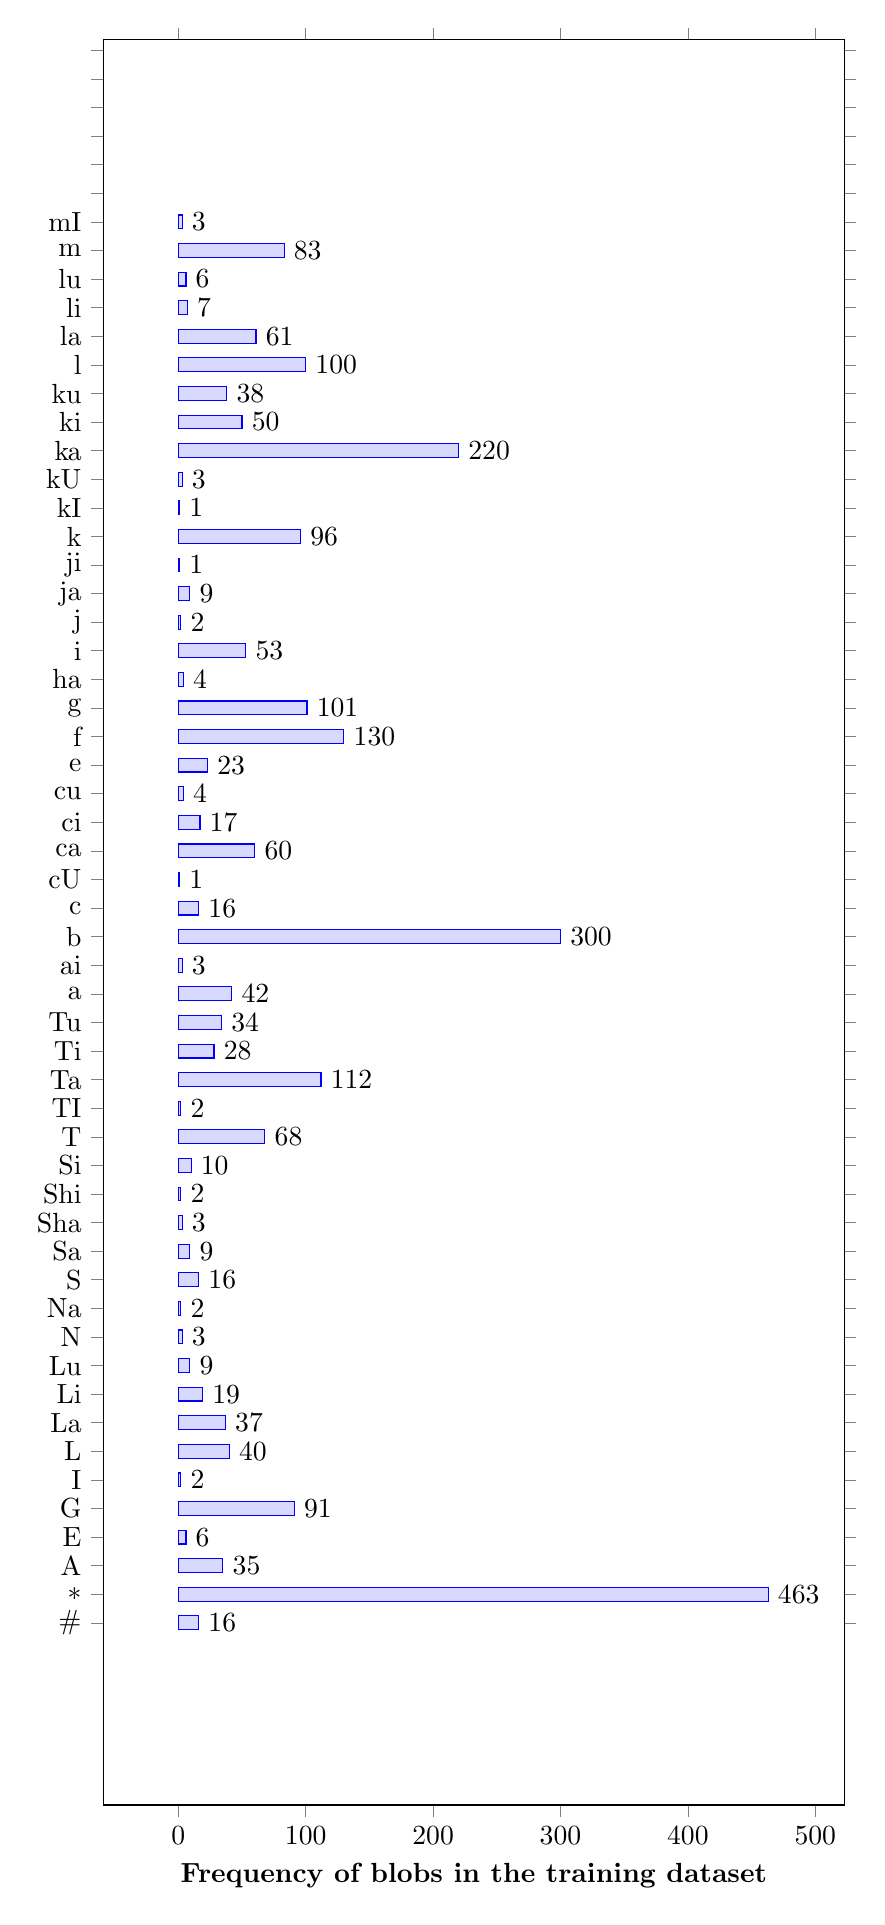
\begin{tikzpicture}[xscale=1, yscale=1]
\begin{axis}
[xbar,width=11cm,height=24cm,bar width=5pt,enlargelimits=0.13,
nodes near coords,nodes near coords
align=horizontal,
point meta=x * 1, % The displayed number.
legend pos=south east,
xlabel=\textbf{Frequency of blobs in the training dataset},
tick align=outside,
xtick={0,100,...,600}, ytick={1,...,155},
 yticklabels={\#,$*$,A,E,G,I,L,La,Li,Lu,N,Na,S,Sa,Sha,Shi,Si,T,TI,Ta,Ti,Tu,a,ai,b,c,cU,ca,ci,cu,e,f,g,ha,i,j,ja,ji,k,kI,kU,ka,ki,ku,l,la,li,lu,m,mI}
]
\addplot[draw=blue, fill=blue!15] coordinates 
{ (16,1) (463,2) (35,3) (6,4) (91,5) (2,6) (40,7) (37,8) (19,9) (9,10) (3,11) (2,12) (16,13) (9,14) (3,15) (2,16) (10,17) (68,18) (2,19) (112,20) (28,21) (34,22) (42,23) (3,24) (300,25) (16,26) (1,27) (60,28) (17,29) (4,30) (23,31) (130,32) (101,33) (4,34) (53,35) (2,36) (9,37) (1,38) (96,39) (1,40) (3,41) (220,42) (50,43) (38,44) (100,45) (61,46) (7,47) (6,48) (83,49) (3,50)  };
\end{axis}
\end{tikzpicture}


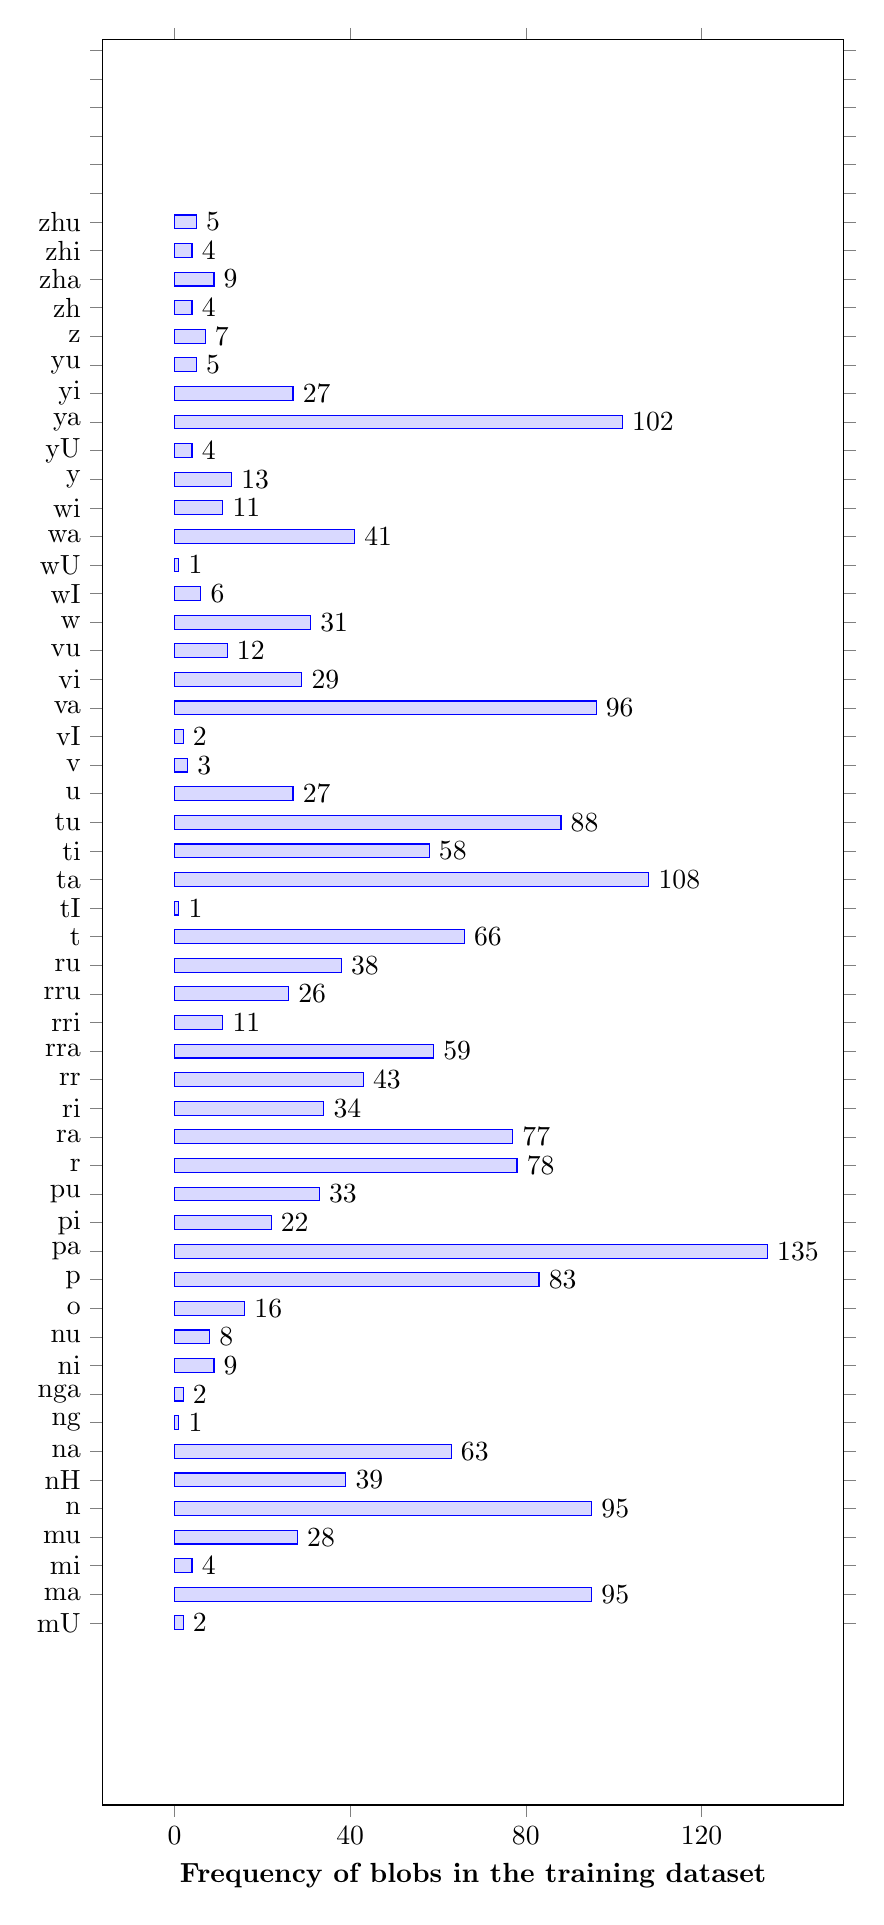
\begin{tikzpicture}[xscale=1, yscale=1]
\begin{axis}
[xbar,width=11cm,height=24cm,bar width=5pt,enlargelimits=0.13,
nodes near coords,nodes near coords
align=horizontal,
point meta=x * 1, % The displayed number.
legend pos=south east,
xlabel=\textbf{Frequency of blobs in the training dataset},
tick align=outside,
xtick={0,40,...,160}, ytick={1,...,155},
 yticklabels={mU,ma,mi,mu,n,nH,na,ng,nga,ni,nu,o,p,pa,pi,pu,r,ra,ri,rr,rra,rri,rru,ru,t,tI,ta,ti,tu,u,v,vI,va,vi,vu,w,wI,wU,wa,wi,y,yU,ya,yi,yu,z,zh,zha,zhi,zhu}
]
\addplot[draw=blue, fill=blue!15] coordinates 
{(2,1) (95,2) (4,3) (28,4) (95,5) (39,6) (63,7) (1,8) (2,9) (9,10) (8,11) (16,12) (83,13) (135,14) (22,15) (33,16) (78,17) (77,18) (34,19) (43,20) (59,21) (11,22) (26,23) (38,24) (66,25) (1,26) (108,27) (58,28) (88,29) (27,30) (3,31) (2,32) (96,33) (29,34) (12,35) (31,36) (6,37) (1,38) (41,39) (11,40) (13,41) (4,42) (102,43) (27,44) (5,45) (7,46) (4,47) (9,48) (4,49) (5,50) };
\end{axis}
\end{tikzpicture}
%\begin{axis}[ legend style={draw=none}] %pgfplot

% \begin{tikzpicture}
% \begin{axis}
% [xbar stacked, stack plots=x, tick align=outside,
% width=8cm, height=16cm, bar width=10pt,
% legend style={cells={anchor=west}}, area legend,
% xlabel=\textbf{Medals Won}, ytick={1,...,5},
% yticklabels={Russia,Netherlands,France,
% South Korea,Japan}]
% \addplot[draw=black,yellow!50!brown]
% coordinates {(1,1) (1,2) (2,3) (2,4) (3,5)};
% \addlegendentry{Gold}
% \addplot[draw=black,white!60!gray]
% coordinates {(1,1) (2,2) (0,3) (0,4) (1,5)};
% \addlegendentry{Silver}
% \addplot[draw=black,orange!70!gray]
% coordinates {(1,1) (0,2) (1,3) (3,4) (3,5)};
% \addlegendentry{Bronze}
% \end{axis}
% \end{tikzpicture}
\subsection{Custom tools}
As part of the project, a blob extractor was developed. It can extract the blob based on the bounding
box information given by tesseract. The ground truth was generated with the help of
an handy interface developed in PyGTK.
  \begin{figure}\centering
\includegraphics[scale=0.3]{./img/blobs} 
  \caption{Sample output after preprocessing}\label{BLOBIMG}
\end{figure}


\begin{figure}\centering
\includegraphics[scale=0.5]{./img/train} 
  \caption{Ground truth generation}\label{GRTR}
\end{figure}

\begin{figure}\centering
\includegraphics[scale=0.3]{./img/model} 
  \caption{Model presented to the recognition engine}\label{MODEL}
  \end{figure}

\begin{figure}\centering
\includegraphics[scale=0.7]{./img/model_gen} 
  \caption{Model generation uses one instance of each of these class}\label{MGEN}
  \end{figure}

\subsection{Elusive samples}
We inspected sample blobs for hierarchal classification. Here are some of the elusive cases
It is called so because noise or improper segmentation makes them stray blobs. Normal contour 
for class 'ya' is one. But in the figure \ref{ESAM} it is three. 
\begin{center}
\begin{figure}\centering

% \begin{tabular}{ | c | c |}
\begin{tabular}{ cc }
% \hline
\includegraphics[scale=0.4]{./img/ya} &

\includegraphics[scale=0.4]{./img/nu} \\ 
% \hline
\includegraphics[scale=0.4]{./img/tu} &
\includegraphics[scale=0.4]{./img/la} \\
% \hline
\end{tabular}


  \caption{Some sample elusive contour from dataset}\label{ESAM}
\end{figure}
\end{center}
\subsection{Confusion matrix}
The confusion matrix is generated with the help of ground truth and some handy shell scripts.
\begin{figure}\centering
\includegraphics[scale=0.7]{./img/confuse}
  \caption{Sample confusion matrix}\label{CONF}
\end{figure}
\subsection{Statistics}
The results are based on training and testing dataset generated as part of this project. It is a
comparison of supervised and unsupervised technique for character recognition. It should be noted that
tesseract doesn't perform perfect segmentation as expected because of touching characters. 
So junk and improper segmentation of blobs are removed from training and testing dataset. 
However, there are some stray characters in the dataset due to the reason stated above. So the 
accuracy is calculated excluding the stray characters.
\begin{table}[!t]\center
% \scriptsize

\begin{tabular}{ | l | l | l | l | l | l | l |}
\hline
& & &  \multicolumn{2}{|c|}{Samples}&\multicolumn{2}{|c|}{Accuracy} \\ \hline
S.No & Method & Features &  Training &Testing & Training & Testing \\ \hline
1* & SVMTC & 555 & 4201 & 4067 & 75 & $<$ 44 (3 classes) \\ \hline
2** & RPT & 1000 & 155 classes& 4201 & 98 & 59 \\
\hline
\end{tabular}
\caption{Recognition result based on SVMTC and RPT } \label{RES}
\end{table}
%         \begin{itemize}
% 	  \item Legend
%   \item *Structural and Statistical features (SVM trainer and classifier is used for classification)
% \item **Random Projection (L2-norm is used for recognition)
%       \end{itemize}
         % Chapter 6
\chapter{Application and Conclusion}


\section{Application}
% \subsection{Parallel corpus}
OCR system is useful for creating volume of corpus by converting existing scanned document into 
plain text. It can also be used for creating encyclopedia from existing old documents. Since  
multilingual encyclopedia can serve as parallel corpus, OCR system would be a handy tool 
for creating dataset from existing paperback encyclopedia. Much of the WWW document images would be 
useful only if it can be indexed because only then it becomes searchable. So OCR plays a major 
role there too. OCR system can also be used in post office where handwritten address is converted into digital format for efficient storage and retrieval. Apart from these examples, OCR system can be 
used anywhere when there is need to convert document image to text.

% \subsection{Post office}


\section{Conclusion and Future enhancement}
In this work, we are presenting a comparative study of recognition based on supervised and 
unsupervised learning.  The former is based on SVM based training and classification(SVMTC) and the
later is based on Random Projection Technique(RPT).Overall, RPT gives better results than
SVMTC. 
The accuracy of recognition can be improved based on hierarchal classification. In order to deal 
with similar characters, nearest neighbor search can be carried out. At the word level, the recognition
can be improved by making use of a dictionary. Finally, all the associated scripts and datasets are made available at \url{https://github.com/pradeepmathesh/tocr} for future enhancement.         % Chapter 7
\addcontentsline{toc}{chapter}{References}
\begin{thereferences}{100}

\bibitem{krish}
V. Krishnamoorthy, "OCR Software for Printed Tamil Text", 
\emph{Proceedings of Tamil Internet 2002}, pp. 99-101, 2002

\bibitem{anbu}
Anbumani Subramanian and Bhadri Kubendran, "Optical Character Recognition of Printed Tamil Characters",\url{http://www.angelfire.com/in/anbu/vt/tamilocr/},(Accessed on: December 2011)

\bibitem{seetha}
Seethalakshmi et.al, "Optical Character Recognition for printed Tamil text using Unicode",\emph{Journal of Zhejiang University Science}, pp. 1297, Sept.10, 2005

\bibitem{jaga1}
Jagadeesh et.al,"Accuracy Augmentation of Tamil OCR Using Algorithm Fusion",\emph{International Journal of Computer Science and Network Security}, VOL.8 No.5, pp.51, May 2008

\bibitem{jaga2}
Jagadeesh et.al,"A Comparative Study of Optical Character Recognition for Tamil Script",\emph{European Journal of Scientific Research}, Vol.35 No.4, pp.570-582, 2009


  \bibitem{lauer}
F. Lauer, "MSVMpack: a Multi-Class Support Vector Machine Package",
\url{http://www.loria.fr/~lauer/MSVMpack,2011},(Accessed on: January 2012)
   
  \bibitem{bresson}
  Xavier Bresson, "A Short Guide on a Fast Global Minimization Algorithm for Active Contour Models", Preprint, April 22, 2009

\bibitem{shi}
Qinfeng Shi, "Rapid Face Recognition Using Hashing", Preprint, 2009
      
\bibitem{dileep}
Dinesh Dileep, "A feature extraction technique based on character geometry for character recognition",
\url{http://www.ece.iisc.ernet.in/~dileep}, 2008,(Accessed on: December 2011)

\bibitem{smith}
Ray Smith, "An Overview of the Tesseract OCR Engine", \emph{IEEE Trans. on Image Processing}, 2007

\bibitem{flusser1}
Jan Flusser and Tomas Suk, "On the Calculation of Image Moments",\emph{Pattern Recognition Letters}, 
January 1999


\bibitem{flusser2}
Jan Flusser et.al,\emph{Moments and Moment Invariants in Pattern Recognition}, 2009

\bibitem{praveen}
Praveen Krishnan, "Preprocessing Algorithms for Tamil
Optical Character Recognition", Master's Thesis, Amrita Vishwa Vidyapeetham, CEN, 2011

\bibitem{amy}
Amy Alison Winder, "Extending the page segmentation algorithms
of the ocropus documentation layout analysis system", Master's Thesis, Boise state university, Department of CS, July 2010

\bibitem{wik1}
SVM - Wikipedia, the free encyclopedia, "\url{http://en.wikipedia.org/wiki/SVM}", (Accessed on: July
2011). 

\bibitem{wik2}
Active contour model - Wikipedia, the free encyclopedia, "\url{http://en.wikipedia.org/wiki/Active_contour_model}", (Accessed on: July 2011). 

% \bibitem{GIT}
% https://github.com/pradeepmathesh/tocr




\end{thereferences}
\appendix

\chapter{Appendix}

\section{Character classes in Tamil OCR}\label{CSET}
The following list presents the character classes in Tamil OCR along with its transliterated mnemonic.
Classes are transliterated for convenience.
\includepdf[pages=-]{tamilset.pdf}
% \section{Complete confusion analysis for RPT based classification}
% \includepdf[pages=-]{hyperres.pdf}


\end{spacing}
                        % example of figs and tables and inclusion of pdf.

%%%%%%%%%%%%%%%%%%%%
% Concluding Pages %
%%%%%%%%%%%%%%%%%%%%%%%%%%%%%%%%%%%%%%%%%%%%%%%%%%%%%%%%%%%%%%%%%%%%%%%%%%%%%%%%

% Bibliography or References, REQUIRED

% If using bibtex, create or modify the refs.bib file
% and use (uncomment) the following three lines.
%\bibliographystyle{plain}     %You may prefer \bibliographystyle{alpha}
%\addcontentsline{toc}{chapter}{\bibname}
%\bibliography{refs}

% If using the ``thereference'' environment instead, modify the ref.tex file
% and use the following line


% If including appendices, uncomment the following lines,
% adding more includes if needed.
%\StartAppendix
%\include{AppendixA}         % Example of how to include an appendix

%\include{vitae}         % Curriculum Vitae      REQUIRED

%%%%%%%%%%%%%%%%%%%%%%%%%%%%%%%%%%%%%%%%%%%%%%%%%%%%%%%%%%%%%%%%%%%%%%%%%%%%%%%%

\end{document}
